\section{Heating Loop (\emph{HeatSys1}) - Boiler}\label{heating-loop-heatsys1---boiler}

The Heating loop is constructed by using a \emph{PlantLoop} object. It uses an electric boiler to (modeled by using a \emph{Boiler:HotWater} object class) to supply hot water to the five heating coils placed in the five zones of the building (modeled by using a \emph{Coil:Heating:Water} object class). Therefore, the supply side of the loop contains the hot water boiler and the demand side contains a total of six heating coils. The loop is operated by using plant equipment operation schemes, and schedules. ~Refer to Figure~\ref{fig:simple-line-diagram-for-the-heating-loop} for a simple diagram of the Condenser Loop.

\begin{figure}[hbtp] % fig 74
\centering
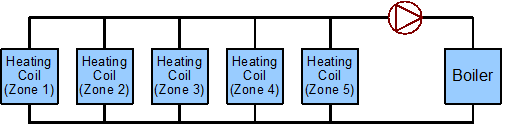
\includegraphics[width=0.9\textwidth, height=0.9\textheight, keepaspectratio=true]{media/image074.png}
\caption{Simple line diagram for the heating loop \protect \label{fig:simple-line-diagram-for-the-heating-loop}}
\end{figure}

\subsection{Flowcharts for the Heating Loop Input Process}\label{flowcharts-for-the-heating-loop-input-process}

This series of flowcharts serve as a guide for identifying and inputting the Heating loop and its components into the input file. The EnergyPlus line diagram for this loop is provided in Figure~\ref{fig:energyplus-line-diagram-for-the-heating-loop}. A simple flowchart for the separation of the half loops is provided in Figure~\ref{fig:simple-flow-chart-for-separation-on-half-002}.

\begin{figure}[hbtp] % fig 75
\centering
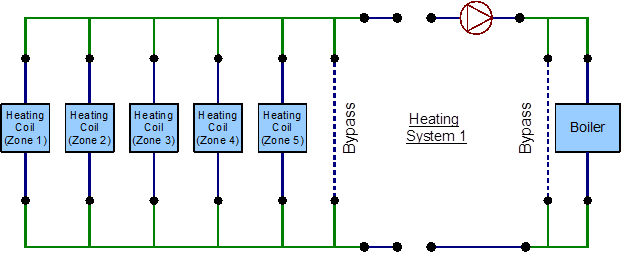
\includegraphics[width=0.9\textwidth, height=0.9\textheight, keepaspectratio=true]{media/image075.png}
\caption{EnergyPlus line diagram for the heating loop \protect \label{fig:energyplus-line-diagram-for-the-heating-loop}}
\end{figure}

\begin{figure}[hbtp] % fig 76
\centering
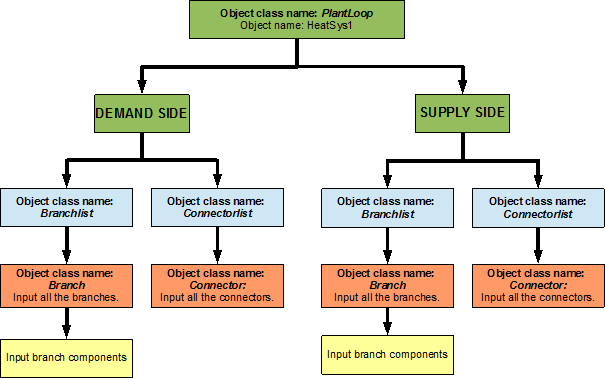
\includegraphics[width=0.9\textwidth, height=0.9\textheight, keepaspectratio=true]{media/image076.png}
\caption{Simple flow chart for separation on half loops in the heating loop \protect \label{fig:simple-flow-chart-for-separation-on-half-002}}
\end{figure}

\subsubsection{Heating Loop Supply Side Construction}\label{heating-loop-supply-side-construction}

The main components on the supply side half loop for the Heating Loop are the hot water boiler that generates hot water and the variable speed pump that circulates the hot water through the loop. This half loop supplies hot water to five heating coils on the demand side half loop. The supply side half loop contains four components, four branches, eight nodes, and one splitter-mixer pair. The EnergyPlus line diagram for the Primary Cooling loop supply side is provided in Figure~\ref{fig:energyplus-line-diagram-for-the-supply-side-004}. The flowchart for supply side branches and components is provided in Figure~\ref{fig:flowchart-for-heating-loop-supply-side-branches-and}. The flowchart for supply side connectors is provided in Figure~\ref{fig:flowchart-for-heating-loop-supply-side-connectors}.

\begin{figure}[hbtp] % fig 77
\centering
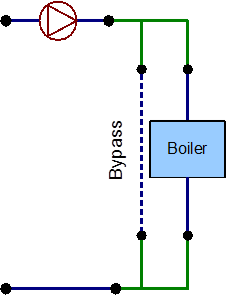
\includegraphics[width=0.9\textwidth, height=0.9\textheight, keepaspectratio=true]{media/image077.png}
\caption{EnergyPlus line diagram for the supply side of the heating loop \protect \label{fig:energyplus-line-diagram-for-the-supply-side-004}}
\end{figure}

\begin{figure}[hbtp] % fig 78
\centering
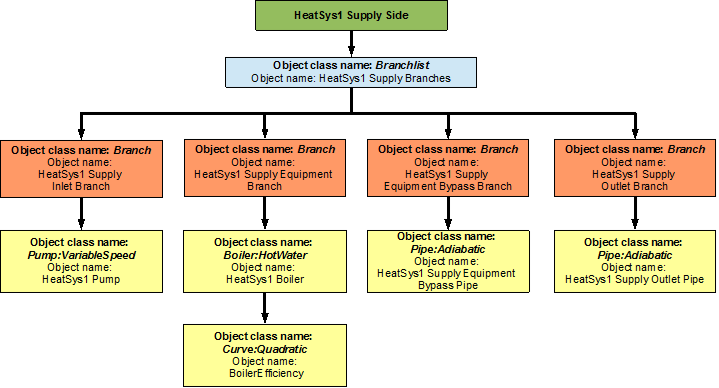
\includegraphics[width=0.9\textwidth, height=0.9\textheight, keepaspectratio=true]{media/image078.png}
\caption{Flowchart for heating loop supply side branches and components \protect \label{fig:flowchart-for-heating-loop-supply-side-branches-and}}
\end{figure}

\begin{figure}[hbtp] % fig 79
\centering
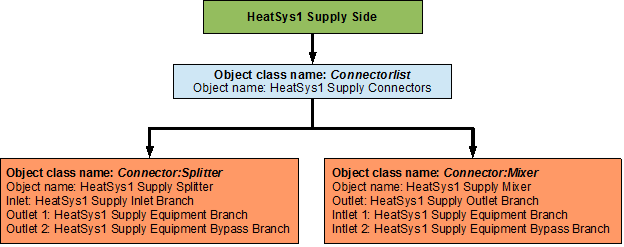
\includegraphics[width=0.9\textwidth, height=0.9\textheight, keepaspectratio=true]{media/image079.png}
\caption{Flowchart for heating loop supply side connectors \protect \label{fig:flowchart-for-heating-loop-supply-side-connectors}}
\end{figure}

\subsubsection{Heating Loop Demand Side Construction}\label{heating-loop-demand-side-construction}

The demand side half loop contains five heating coils that heat the air in the different zones of the building by using the hot water that is supplied by the hot water boiler. This side of the loop also has sixteen nodes, eight components, eight branches, and one splitter-mixer pair. An EnergyPlus schematic for the demand side is provided in Figure~\ref{fig:energyplus-line-diagram-for-the-demand-side-004}. The flowchart for demand side branch definition is provided in Figure~\ref{fig:flowchart-for-heating-loop-demand-side-branches-and}. The flowchart for the demand side connectors is provided in Figure~\ref{fig:flowchart-for-heating-loop-demand-side-connectors}.

\begin{figure}[hbtp] % fig 80
\centering
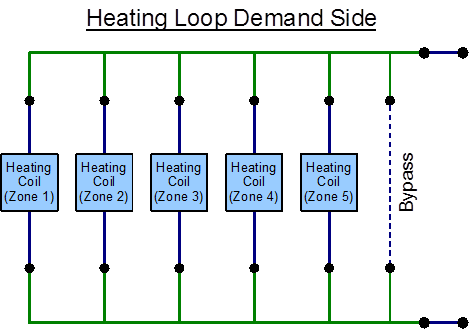
\includegraphics[width=0.9\textwidth, height=0.9\textheight, keepaspectratio=true]{media/image080.png}
\caption{EnergyPlus line diagram for the demand side of the heating loop \protect \label{fig:energyplus-line-diagram-for-the-demand-side-004}}
\end{figure}

\begin{figure}[hbtp] % fig 81
\centering
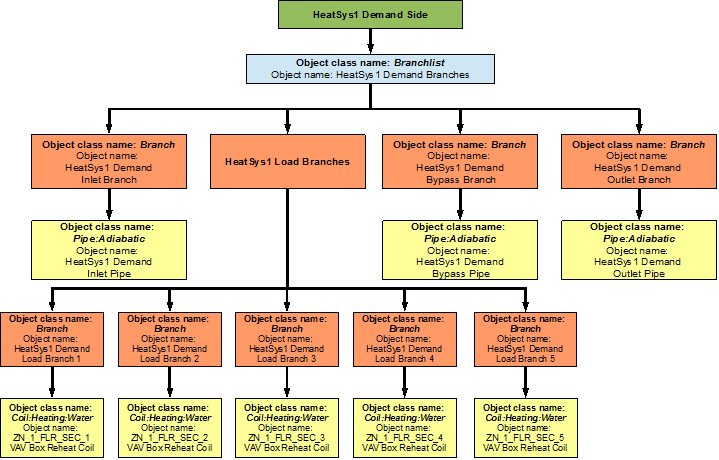
\includegraphics[width=0.9\textwidth, height=0.9\textheight, keepaspectratio=true]{media/image081.png}
\caption{Flowchart for heating loop demand side branches and components \protect \label{fig:flowchart-for-heating-loop-demand-side-branches-and}}
\end{figure}

\begin{figure}[hbtp] % fig 82
\centering
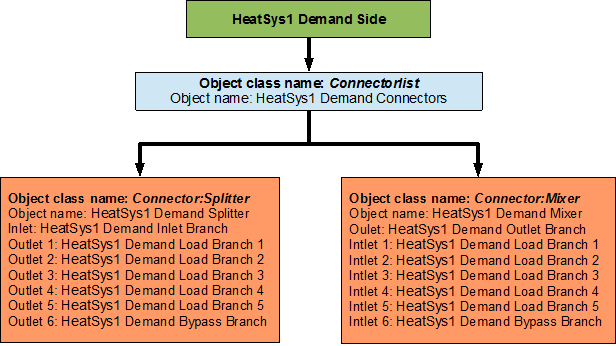
\includegraphics[width=0.9\textwidth, height=0.9\textheight, keepaspectratio=true]{media/image082.png}
\caption{Flowchart for heating loop demand side connectors \protect \label{fig:flowchart-for-heating-loop-demand-side-connectors}}
\end{figure}

\subsection{Flowcharts for Heating Loop Controls}\label{flowcharts-for-heating-loop-controls}

The Heating Loop is operated by using set-points, plant equipment operation schemes and schedules.

\subsubsection{Heating Loop Schedules}\label{heating-loop-schedules}

The flowchart for Primary Heating loop schedule definition is provided in Figure~\ref{fig:flowchart-for-heating-loop-schedules}. The Heating Loop uses three different schedules to operate properly. \emph{PlantOnSchedule} is a compact schedule that uses a discrete \emph{ScheduleTypeLimit} (\emph{On/Off)} which defines that the value of ON is 1 and that of Off is 0. This plant loop also uses another compact schedule named \emph{HW Loop Temp Schedule} to declare that the temperature at the heating loop outlet and the boiler outlet to be 82 degrees Celsius. This schedule uses a schedule type limit named \emph{Temperature,} which defines the loop upper and lower temperature limits. The compact schedule \emph{ALWAYS\_ON} dictates that the boiler and the cooling coils are On at all times of the day. This schedule uses the \emph{ScheduleTypeLimit (Fraction)} to set the fractional flow rate of the components to 1.

\begin{figure}[hbtp] % fig 83
\centering
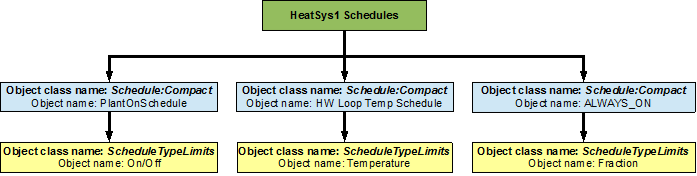
\includegraphics[width=0.9\textwidth, height=0.9\textheight, keepaspectratio=true]{media/image083.png}
\caption{Flowchart for heating loop schedules \protect \label{fig:flowchart-for-heating-loop-schedules}}
\end{figure}

\subsubsection{Heating Loop Plant Equipment Operation Schemes}\label{heating-loop-plant-equipment-operation-schemes}

The \emph{PlantEquipmentOperationschemes} object uses the \emph{PlantOnSchedule} and the \emph{HeatSys1 Operation Scheme} objects to set the range of the demand loads for which the boiler is operated during the simulation period. Operation schemes are especially useful and crucial when using multiple active components but it is required to enter set up a plant equipment operation scheme for every \emph{PlantLoop} that is used in a system. A flowchart detailing the heating loop plant equipment operation scheme is provided in Figure~\ref{fig:flowchart-for-heating-loop-plant-equipment-operation}.

\begin{figure}[hbtp] % fig 84
\centering
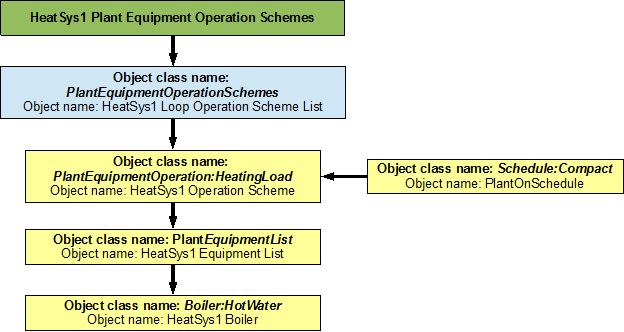
\includegraphics[width=0.9\textwidth, height=0.9\textheight, keepaspectratio=true]{media/image084.png}
\caption{Flowchart for heating loop plant equipment operation schemes \protect \label{fig:flowchart-for-heating-loop-plant-equipment-operation}}
\end{figure}

\subsubsection{Heating Loop Setpoints}\label{heating-loop-setpoints}

The \emph{HeatSys1 Loop Setpoint Manager} uses the \emph{HW Loop Temp Schedule} to set a temperature control point at the \emph{HeatSys1 Supply Outlet Node}. This setpoint allows the program to control the temperature (set to 82 degrees Celsius) at the node by operating the components in the Heating loop. The Heating Loop also uses another schedule (\emph{HeatSys1 Boiler Setpoint Manager)} to set the temperature of the boiler outlet to 82 degrees Celsius. If the \emph{HeatSys1 Boiler Setpoint Manager} is not entered the program assumes the overall loop setpoint for the boiler outlet node. Since, setpoint managers are high-level control objects, their usefulness is realized in much more complex systems, where multiple nodes have to be monitored in order to operate the system properly. A flowchart for heating loop setpoints is provided in Figure~\ref{fig:flowchart-for-heating-loop-setpoints}.

\begin{figure}[hbtp] % fig 85
\centering
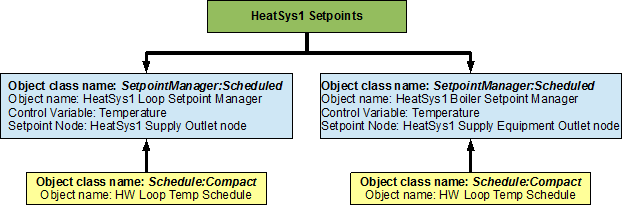
\includegraphics[width=0.9\textwidth, height=0.9\textheight, keepaspectratio=true]{media/image085.png}
\caption{Flowchart for heating loop setpoints \protect \label{fig:flowchart-for-heating-loop-setpoints}}
\end{figure}

\subsubsection{Heating Loop Sizing}\label{heating-loop-sizing}

The Heating Loop is sized such a way that the design loop exit temperature is 82.0 degrees Celsius, and the loop design temperature difference is 11.0 degrees Celsius. A flowchart for the chilled water loop sizing is provided in Figure~\ref{fig:flowchart-for-heating-loop-sizing}.

\begin{figure}[hbtp] % fig 86
\centering
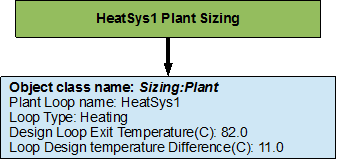
\includegraphics[width=0.9\textwidth, height=0.9\textheight, keepaspectratio=true]{media/image086.png}
\caption{Flowchart for heating loop sizing \protect \label{fig:flowchart-for-heating-loop-sizing}}
\end{figure}
